%%%%%%%%%%%%%%%%%%%%%%%%%%%%%%%%%%%%%%%%%%%%%%%%%%%%%%%%%%%%%%%%%%%%%%%%%%%%%
\chapter{Introduction}\label{chap:introduction}
%%%%%%%%%%%%%%%%%%%%%%%%%%%%%%%%%%%%%%%%%%%%%%%%%%%%%%%%%%%%%%%%%%%%%%%%%%%%%
\chapterstart

This template shall provide some considerations and text examples for your Master's thesis.

% example for a named paragraph
\paragraph{Background.}
Describe the background, the prerequisites for your work \ldots


\paragraph{Objective.}
The aim of this master's thesis is \ldots


\paragraph{Terms and definitions.}
Technical terms \ldots\ abbreviations are summarised at the end (in~``\nameref{chap:acronyms}''), e.g.\ \ac{ABI} or \ac{MITM}. If \ac{ABI} is referenced again, only the acronym is printed (as hyperlink though).

For literature research use e.g. \citetitle{acm:diglibrary} \parencite{acm:diglibrary} or \citetitle{ieee:xplore} \parencite{ieee:xplore} as available from the FH JOANNEUM Libary web page.

Harvard citation style is implemented in this template: \citet{Batina:2011}, \citet{Fernandez-Mir:2011}, \citet{Li:2008}


\section{Some \LaTeX{} Basics}
%----------------------------------------------------------------------------
This section is a \textit{really very short} summary of \LaTeX\ features. Do not forget to remove it after finishing your thesis.

Here you have an included graphic (figure~\ref{fig:engine}).

\begin{figure}[h]
\centering
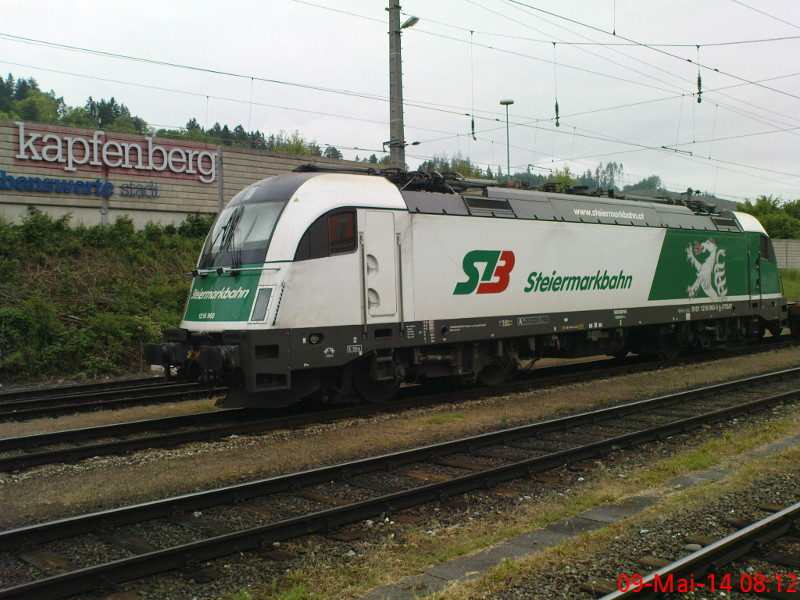
\includegraphics[keepaspectratio,width=0.8\textwidth]
{images/engine}
\caption{Train engine in Kapfenberg}
\label{fig:engine}
\end{figure}

Code listings require the \textit{listings} package which, in turn, requires some settings\footnote{\ldots because the defaults do not fit all purposes}; see command \verb+\lstset{}+ in preamble of this template. Additionally the package \textit{courier} should be used because the defaults do not provide for proper syntax highlighting.

\lstset{caption=Main programme, basicstyle=\small\ttfamily, label=lst:main, language=C}
%	basewidth={0.55em}, fontadjust}	% adjust these for more appealing appearance
\begin{lstlisting}
void main(int argc, char *argv[])
{
  printf("Hello world!");
}
\end{lstlisting}

In order to see what's possible -- here are two fancy tables: \ref{tab:olive} and \ref{tab:grey}.

\begin{center}
\begin{table}[h]
\begin{tabular}{|l|l|l|l|}\hline
\rowcolor{olivegreen30}
\textcolor{white}{\textbf{Version}}
		&
		\textcolor{white}{\textbf{Description}}	&
							\textcolor{white}{\textbf{Author(s)}}	&
																\textcolor{white}{\textbf{Date}}\\\hline
1.0		& Initial				& Ohrt					& July 15, 2014\\\hline
1.1		& Filled section ``Open Issues''	& Ohrt					& July 16, 2014\\\hline
1.2		& Added section ``Restrictions''	& Ohrt					& September 15, 2014\\\hline
\end{tabular}
\caption{Olive green heading} \label{tab:olive}
\end{table}

\begin{table}[h]
\begin{tabular}{ l | l }
\rowcolor{gray20}\textbf{Error}	& \textbf{Solution} \\
\rowcolor{gray5}Java.lang.OutOfMemoryError: PermGen space
									& -XX:MaxPermSize=1024M \\
\rowcolor{gray5}\textit{(32-/64-bit issue)}
									& \\
\rowcolor{gray20}Error occurred during initialization of VM \textit{or}
									& increase or remove -Xms value \\
\rowcolor{gray20}Could not reserve enough space for object heap
									& e.g.\ -Xms128m -Xmx512m \\
\rowcolor{gray20}					& \small{(Eclipse default:}\\
\rowcolor{gray20}					& \small{-Xms40m -Xmx512m)} \\
\end{tabular}
\caption{A grey table} \label{tab:grey}
\end{table}
\end{center}

View also the preamble of this file for explanations.

Here is a reference to listing~\ref{lst:main}.

% next chapter: start at right side, if two-sided; else just flush page
\chapterend
